\section{Thermodynamics}

\paragraph{Functions of State}
A quantity $f$ is a function of state if its equilibrium value is a function of the equilibrium values of the variables describing the state.

\paragraph{Intensive and Extensive Variables}
Intensive variables do not depend on the size of the system, whereas extensive variables do. Examples of the former are pressure and temperature, and examples of the latter are volume and total energy.

\paragraph{Heat}
Heat is the flow of energy.

\paragraph{Internal Energy}
The internal energy $U$ of a system is the sum of the energy of all the internal degrees of freedom of a system.

\paragraph{Quasistatic Processes}
A process is quasistatic if the system is in equilibrium at each point during the process. Reversible processes must be performed quasistatically.

\paragraph{Work}
The work performed on a system is a mechanical addition of energy. It is generally of the form
\begin{align*}
	\din{W} = X\dd{x},
\end{align*}
where $X$ is an intensive generalized force and $x$ an extensive generalized displacement. For gases, around which most of the following discussions will focus, we have $X = -p$ and $x = V$. Other examples would include elastic rods, with $X$ as the rod tension and $x$ as its extension, or liquid surfaces, with $X$ as the surface tension and $x$ as the surface area.

This might of course seemingly imply that work is indeed a function of state - after all, it seems to be an exact differential. The flaw in this argument lies in the work only looking like this when performed in a reversible manner.

\paragraph{The First Law}
Energy is conserved and heat and work are both forms of energy. In mathematical form:
\begin{align*}
\dd{U} = \din{Q} + \din{W}.
\end{align*}
This implies the convention that positive differentials correspond to energy supplied to the system.

\paragraph{The Second Law of Thermodynamics}
The second law comes in two different statements:
\begin{itemize}
	\item \textbf{Clausius' statement:} No process is possible whose sole result is the transfer of heat from a colder to a hotter body.
	\item \textbf{Kelvin's statement:} No process is possible whose sole result is the complete conversion of heat into work.
\end{itemize}

\paragraph{Equivalence of Statements}
Consider two heat reservoirs. We want to show that the existence of a system that violates one statement implies the existence of a system that violates the other.

To prove that Clausius' statement implies Kelvin's, we introduce a Clausius violater which can transfer heat from a cold to a hot reservoir. Suppose that the violator transfers a heat $Q_{\text{l}}$ between the reservoirs and introduce a heat engine which produces work while transferring heat $Q_{\text{h}}$ from the hot reservoir and leaving $Q_{\text{l}}$ in the cold reservoir. The combination of these two systems thus convert heat $Q_{\text{h}} - Q_{\text{l}}$ to work with no other results, violating Kelvin's statement.

To prove that Kelvin's statement implies Clausius', we introduce a Kelvin violater which can convert heat directly to work. Suppose that the violator converts a heat $W$ into work, and let this work run a reverse heat engine between the reservoirs taking heat $Q_{\text{l}}$ from the cold reservoir and leaving heat $Q_{\text{h}}$ in the cold reservoir. The combination of these two systems thus transfer heat $Q_{\text{l}}$ from the cold reservoir to the hot reservoir with no other results, violating Kelvin's statement.

\paragraph{Ideal Gases}
Consider a gas with negligible internal interactions. For such a gas experiments have revealed
\begin{align*}
	pV = nRT.
\end{align*}

\paragraph{Heat Capacity of a Gas}
For a gas we have
\begin{align*}
	\dd{U} = \fix{\pdv{U}{T}}{V}\dd{T} + \fix{\pdv{U}{V}}{T}\dd{V},
\end{align*}
as $U$ is a  function of state. The subscript indicates which variables are constant when the derivatives are computed. The first law gives
\begin{align*}
	\din{Q} = \fix{\pdv{U}{T}}{V}\dd{T} + \left(\fix{\pdv{U}{V}}{T} + p\right)\dd{V}.
\end{align*}
Heat capacitites are defined as derivatives of $Q$ with respect to temperature. We thus obtain
\begin{align*}
	C_{V} = \fix{\pdv{Q}{T}}{V} = \fix{\pdv{U}{T}}{V},\ C_{p} = \fix{\pdv{Q}{T}}{p} = \fix{\pdv{U}{T}}{V} + \left(\fix{\pdv{U}{V}}{T} + p\right)\fix{\pdv{V}{T}}{p}.
\end{align*}
In particular, we have for an ideal gas (where there are no interactions, and the internal energy thus does not depend on the colume) that
\begin{align*}
	C_{p} = C_{V} + p\frac{nR}{p} = C_{V} + nR.
\end{align*}
Heat capacities may be derived similarly for other kinds of systems.

\paragraph{Molar Heat Capacities}
Molar heat capacities, denoted with a small $c$, are heat capacities per mole.

\paragraph{Adiabatic Index}
The adiabatic index is defined as
\begin{align*}
	\gamma = \frac{C_{p}}{C_{V}}.
\end{align*}

\paragraph{Processes on Ideal Gases}
Processes performed on ideal gases may be characterized as
\begin{itemize}
	\item isobaric, where the pressure is constant.
	\item isochoric, where the volume is constant.
	\item isothermal, where the temperature is constant. For such processes, we also have that $pV$ is constant.
	\item adiabatic, where the gas does not exchange heat with its surroundings. For such processes, we have
	\begin{align*}
		\din{Q}               &= \dd{U} - p\dd{V} = 0, \\
		C_{V}\dd{T}           &= \frac{nRT}{V}\dd{V}, \\
		\frac{C_{V}}{T}\dd{T} &= \frac{nR}{V}\dd{V} = \frac{C_{p} - C_{V}}{V}\dd{V}, \\
		\ln{\frac{T}{T_{0}}}  &= (\gamma - 1)\ln{\frac{V}{V_{0}}},
	\end{align*}
	meaning that $TV^{\gamma - 1}$ is constant. This may of course be re-expressed in terms of other combinations of thermodynamic variables.
\end{itemize}

\paragraph{The Carnot Cycle}
Consider a machine performing work based on the energy transfer between two heat reservoirs. One way to extract the energy is by using a Carnot process, which uses an ideal gas. The cycle connects four different points in a $pV$ diagram with two adiabatics and two isothermals.

More specifically, introduce the two heat reservoirs $T_{\text{h}} > T_{\text{l}}$ and the notation for each step according to figure \ref{fig:carnot}.
\begin{figure}[!ht]
	\centering
	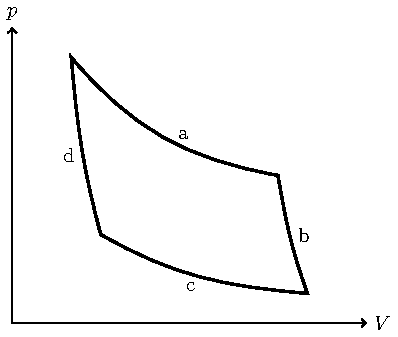
\includegraphics[width = 0.5\textwidth]{./Images/carnot.pdf}
	\caption{Schematic of a Carnot cycle.}
	\label{fig:carnot}
\end{figure}

During step a, the gas expands isothermally, and we have
\begin{align*}
	\Delta U = 0,\ Q = W = nRT_{\text{h}}\ln{\frac{V_{\text{b}}}{V_{\text{a}}}}.
\end{align*}

During step b, the gas expands adiabatically, and we have
\begin{align*}
	Q = 0,\ W = \Delta U = C_{V}(T_{\text{l}} - T_{\text{h}}).
\end{align*}

During step c, the gas compresses isothermally, and we have
\begin{align*}
	\Delta U = 0,\ Q = W = nRT_{\text{l}}\ln{\frac{V_{\text{d}}}{V_{\text{c}}}}.
\end{align*}

During step b, the gas compresses adiabatically, and we have
\begin{align*}
	Q = 0,\ W = \Delta U = C_{V}(T_{\text{h}} - T_{\text{l}}).
\end{align*}

We use the previously derived expressions for adiabatic processes to write
\begin{align*}
	T_{\text{h}}V_{a}^{\gamma - 1} = T_{\text{l}}V_{d}^{\gamma - 1},\ T_{\text{h}}V_{b}^{\gamma - 1} = T_{\text{l}}V_{c}^{\gamma - 1}.
\end{align*}
Thus we obtain for the isothermal compression that
\begin{align*}
	Q = nRT_{\text{l}}\ln(\frac{\left(\frac{T_{\text{h}}}{T_{\text{l}}}\right)^{\frac{1}{\gamma - 1}}V_{a}}{\left(\frac{T_{\text{h}}}{T_{\text{l}}}\right)^{\frac{1}{\gamma - 1}}V_{b}}) = nRT_{\text{l}}\ln(\frac{V_{a}}{V_{b}}),
\end{align*}
and thus $\frac{\abs{Q}}{T}$ is constant for the two heat-exchanging steps.

\paragraph{Efficiency}
The efficiency of a machine has various definitions, but the general definition is the ratio between the energy you get out and the energy you put in.

\paragraph{Carnot's Theorem}
No heat engine working between two heat reservoirs is more efficient than a Carnot engine.

To prove this, suppose that you create an engine producing the same work $W$ as a Carnot heat engine, but for an energy $Q'$ as opposed to the energy $Q$ needed to run the Carnot engine. Now let your new engine be used to power a reversed Carnot engine. As the process must be performed cyclically, the statement that this new engine is more efficient is expressed as
\begin{align*}
	\frac{W}{Q'} > \frac{W}{Q} \implies Q > Q'.
\end{align*}
During the process each engine gives off some heat $Q_{\text{l}}$ to the cold reservoir. The first law of thermodynamics implies
\begin{align*}
	W = Q' - Q_{\text{l}}' = Q - Q_{\text{l}}.
\end{align*}
As $Q - Q' > 0$, so is $Q_{\text{l}} - Q_{\text{l}}'$. Now, $Q - Q'$ is the net energy left in the hot reservoir during a cycle and $Q_{\text{l}} - Q_{\text{l}}'$ is the energy extracted from the cold reservoir. The sole result of this process is thus to extract energy from a cold reservoir to a hot one, which violates the second law.

\subparagraph{Corollary}
All reversible heat engines working between two temperatures have the same efficiency as a Carnot engine.

To show this, suppose a Carnot engine is working between two reservoirs and running another engine undoing that process. This other engine cannot be more efficient than the Carnot engine, meaning that it delivers a greater amount of energy to the hot reservoir than the Carnot engine took, violating the second law of thermodynamics. Thus the two engines must have the same efficiency.

\paragraph{Clausius' Theorem}
Consider some arbitrary cyclic process. We can describe this as a sequence of the system being connected to temperatures $T_{i}$, with heats $\din{Q_{i}}$ being supplied at every stage. The total work performed during the cycle is given by
\begin{align*}
	W = \sum\din{Q_{i}}.
\end{align*}
Now suppose that the heat at each point is supplied by a Carnot engine operating between two reservoirs at temperature $T$ and $T_{i}$. Using the constant ratio for Carnot cycles which was derived previously, we have
\begin{align*}
	\frac{\din{Q_{i}}}{T_{i}} = \frac{\din{Q_{i}} + \din{W_{i}}}{T}
\end{align*}
where $\din{W_{i}}$ is the work done by the Carnot engine. This process cannot violate the second law of thermodynamics, hence
\begin{align*}
	W + \sum\din{W_{i}} \leq 0.
\end{align*}
Hence
\begin{align*}
	\sum\din{Q_{i}} + \sum\din{Q_{i}}\left(\frac{T}{T_{i}} - 1\right) = T\sum\frac{\din{Q_{i}}}{T_{i}} \leq 0.
\end{align*}
The temperature $T$ is constant and positive, and can thus be ignored. In the limit of considering the process in a continuous manner, this becomes
\begin{align*}
	\intin{}{}{Q}{\frac{1}{T}} \leq 0.
\end{align*}
This is Clausius' theorem, where equality necessarily holds for a reversible cycle.

\paragraph{Entropy}
As we have seen, the integral
\begin{align*}
	\intin{}{}{Q}{\frac{1}{T}}
\end{align*}
is path independent for a reversible process. We thus define the state function
\begin{align*}
	\dd{S} = \frac{\din{Q}}{T}
\end{align*}
to be the entropy.

\paragraph{The Second Law and Entropy}
Consider two points connected by a reversible and an irreversible process such that the two form a cycle. Clausius' theorem yields
\begin{align*}
	\intin{A}{B}{Q}{\frac{1}{T}} + \intin{B}{A}{Q_{\text{rev}}}{\frac{1}{T}} \leq 0 \implies \intin{A}{B}{Q}{\frac{1}{T}} \leq \intin{A}{B}{Q_{\text{rev}}}{\frac{1}{T}}.
\end{align*}
This holds for two arbitrary points, meaning
\begin{align*}
	\dd{S} \geq \frac{\din{Q}}{T}.
\end{align*}
Considering a thermally isolated system, we obtain
\begin{align*}
	\dd{S} \geq 0.
\end{align*}
This is a restatement of the second law of thermodynamics, and essentially an equilibrium condition for any isolated system.

\paragraph{The First Law and Entropy}
For a reversible process on a gas we obtain
\begin{align*}
	\dd{U} = T\dd{S} - p\dd{V},
\end{align*}
or more generally
\begin{align*}
	\dd{U} = T\dd{S} + X\dd{x}.
\end{align*}
However, as all involved quantities are functions of state, this must hold even if the process in question is irreversible.

\paragraph{The Third Law}
The third law was initially concerned with the issue of determining absolute entropies. Three different statements of the third law were finally coined:

\begin{itemize}
	\item \textbf{Nernst's statement:} Near absolute zero, all reactions in a system in internal equilibrium take place with no change in entropy.
	\item \textbf{Planck's statement:} The entropy of all systems in internal equilibrium is the same at absolute zero, and may be taken to be zero.
	\item \textbf{Simon's statement:} The contribution to the entropy of a system by each aspect of the system which is in internal thermodynamic equilibrium tends to zero when approaching absolute zero.
\end{itemize}

Simon's idea of aspects are based on a closer and closer inspections of a system. Considering a crystal for instance, it can be studied as a macroscopic entity or in terms of the individual atoms comprising it. These are, in turn, built up of nucleons, which are made up of quarks and so on (potentially). Each of these is termed an aspect.

\paragraph{Natural Variables For Internal Energy}
Our restatement of the first law implies that $U$ is most naturally written as a function of $S$ and $x$ (naturally it could be written in terms of other variables too, but you would have to change variables from $S$ and $x$ in order to do that. A switch from $S$ to $T$ would for instance be rewriting $U$ as $U(S(T), x)$). The restatement also implies
\begin{align*}
	\fix{\pdv{U}{S}}{V} = T,\ \fix{\pdv{U}{x}}{S} = X.
\end{align*}

\paragraph{Chemical Potential}
In addition to the dependence of the internal energy on entropy and volume, there is a dependence on the number of particles of type $i$. This is contained in the chemical potential, defined as
\begin{align*}
	\mu_{i} = \fix{\pdv{U}{N_{i}}}{S, x, N_{j}}
\end{align*}
where $j \neq i$. From now on, summation rules will be used for chemical potentials, $i$ will signify all sets of possible values of $i$, and $j\neq i$ may always be assumed to be true unless otherwise specified.

\paragraph{Entropy}
We can re-express the differential of internal energy as a differential of entropy or use the reciprocal and reciprocity theorems to obtain
\begin{align*}
	\dd{S} = \frac{1}{T}\dd{U} - \frac{X}{T}\dd{x}.
\end{align*}
This implies that the entropy is a function of $U$, $x$ and $N_{i}$, as well as
\begin{align*}
	\fix{\pdv{S}{U}}{x, N_{i}} = \frac{1}{T},\ \fix{\pdv{S}{x}}{U, N_{i}} = -\frac{X}{T},\ \fix{\pdv{S}{N_{i}}}{U, x, N_{j}} = -\frac{\mu_{i}}{T}.
\end{align*}

\paragraph{Enthalpy}
%TODO: Continue to rewrite for general systems
The enthalpy is defined as 
\begin{align*}
	H = U + pV.
\end{align*}
We have
\begin{align*}
	\dd{H} = \dd{U} + p\dd{V} + V\dd{p} = T\dd{S} - p\dd{V} + \mu_{i}\dd{N_{i}} + p\dd{V} + V\dd{p} = T\dd{S} + V\dd{p} + \mu_{i}\dd{N_{i}},
\end{align*}
implying that $H$ is a function of $S$, $p$ and $N_{i}$, as well as
\begin{align*}
	\fix{\pdv{H}{S}}{p, N_{i}} = T,\ \fix{\pdv{H}{p}}{S, N_{i}} = V,\ \fix{\pdv{H}{N_{i}}}{S, V,  N_{j}} = \mu_{i}.
\end{align*}

\paragraph{Helmholtz Free Energy}
The Helmholtz free energy is defined as
\begin{align*}
	F = U - TS.
\end{align*}
We have
\begin{align*}
	\dd{F} = \dd{U} - T\dd{S} - S\dd{T} = T\dd{S} - p\dd{V} + \mu_{i}\dd{N_{i}} - T\dd{S} - S\dd{T} = -p\dd{V} - S\dd{T} + \mu_{i}\dd{N_{i}},
\end{align*}
implying that $F$ is a function of $T$, $V$ and $N_{i}$, as well as
\begin{align*}
	\fix{\pdv{F}{T}}{V, N_{i}} = -S,\ \fix{\pdv{F}{V}}{T, N_{i}} = -p,\ \fix{\pdv{F}{N_{i}}}{T, V,  N_{j}} = \mu_{i}.
\end{align*}

\paragraph{Gibbs Free Energy}
The Gibbs free energy is defined as
\begin{align*}
	G = H - TS.
\end{align*}
We have
\begin{align*}
	\dd{G} = \dd{H} - T\dd{S} - S\dd{T} = T\dd{S} + V\dd{p} + \mu_{i}\dd{N_{i}} - T\dd{S} - S\dd{T} = V\dd{p} - S\dd{T} + \mu_{i}\dd{N_{i}},
\end{align*}
implying that $G$ is a function of $T$, $p$ and $N_{i}$, as well as
\begin{align*}
	\fix{\pdv{G}{T}}{p} = -S,\ \fix{\pdv{G}{p}}{T} = V,\ \fix{\pdv{G}{N_{i}}}{T, p,  N_{j}} = \mu_{i}.
\end{align*}

\paragraph{The Grand Potential}
The grand potential is defined as
\begin{align*}
	\GP = F - \mu_{i}N_{i}.
\end{align*}
We have
\begin{align*}
	\dd{\GP} = -p\dd{V} - S\dd{T} + \mu_{i}\dd{N_{i}} - \mu_{i}\dd{N_{i}} - N_{i}\dd{\mu_{i}} = -p\dd{V} - S\dd{T} - N_{i}\dd{\mu_{i}},
\end{align*}
implying that $\GP$ is a function of $V$, $T$ and $\mu_{i}$, as well as
\begin{align*}
	S = - \fix{\pdv{\GP}{T}}{V, \mu},\ p = - \fix{\pdv{\GP}{V}}{T, \mu},\ N_{i} = - \fix{\pdv{\GP}{\mu_{i}}}{T, V, N_{j}}.
\end{align*}

\paragraph{Maxwell Relations}
Using the symmetry of partial derivatives for a state function, one can obtain relations between derivatives of other state functions.

As an example, the derivatives of $F$ are $-S$ and $-p$, computed with respect to $T$ and $V$. This implies
\begin{align*}
	\fix{\pdv{S}{V}}{T} = \fix{\pdv{p}{T}}{V}.
\end{align*}

\paragraph{Consequences of the Third Law}
Now we examine some of the consequences of the third law.

The first consequence is for heat capacities near absolute zero. We have
\begin{align*}
	C = T\pdv{S}{T} = \pdv{S}{\ln{T}} \to 0.
\end{align*}
One might suspect that the first equality implies it (and I don't know why it does not). But the second statement guarantees it somehow, as the third law implies that the entropy is bounded at low temperatures.

A second consequence is for thermal expansion. The third law implies
\begin{align*}
	\fix{\pdv{S}{p}}{T} \to 0
\end{align*}
near absolute zero, which implies
\begin{align*}
	\fix{\pdv{V}{T}}{p} \to 0.
\end{align*}

A third consequence is for ideal systems, such as the ideal gas and non-interacting spin systems. These cannot be ideal at low temperatures, a fact that might be guessed at based on tendencies in their entropies, but can also be justified by the fact that interactions between units in the system can be disregarded at high temperatures, where the ideal models are valid, but not at lower temperatures.

A final consequence is the fact that one cannot cool to $T = 0$ in a finite number of steps, a fact which is not easy to prove rigorously.

\paragraph{Reinterpretation of the Chemical Potential and Grand Potential}
Consider a system of only one kind of particles which is scaled by a factor $\lambda$. The entropy, expressed as a function of $U$, $V$ and $N$ is extensive, yielding that it, too, is scaled by a factor $\lambda$. Let a subscript $\lambda$ denote quantities for a scaled system. We thus have
\begin{align*}
	S_{\lambda} = \lambda S.
\end{align*}
Differentiating with respect to $\lambda$ 
\begin{align*}
	S &= \fix{\pdv{S_{\lambda}}{U_{\lambda}}}{V_{\lambda}, N_{\lambda}}\pdv{U_{\lambda}}{\lambda} + \fix{\pdv{S_{\lambda}}{V_{\lambda}}}{U_{\lambda}, N_{\lambda}}\pdv{V_{\lambda}}{\lambda} + \fix{\pdv{S_{\lambda}}{N_{\lambda}}}{U_{\lambda}, V_{\lambda}}\pdv{N_{\lambda}}{\lambda}.
\end{align*}
Setting $\lambda = 1$ or arguing that temperature is intensive yields that this is equal to
\begin{align*}
	S = \frac{U}{T} + \frac{p}{T} - \frac{\mu}{T}. 
\end{align*}
We can rewrite this as
\begin{align*}
	U - TS + pV = G = \mu N,
\end{align*}
and thus that $\mu$ is the Gibbs free energy per particle. For a system of multiple kinds of particles we instead obtain
\begin{align*}
	G = \mu_{i}N_{i},
\end{align*}
and we now interpret $\mu_{i}$ as the Gibbs free energy per particle of type $i$.

This also implies
\begin{align*}
	\GP = -pV.
\end{align*}

\paragraph{The Gibbs-Duhem Relation}
We have
\begin{align*}
	\dd{\mu_{i}N_{i}} = \mu_{i}\dd{N_{i}} + N_{i}\dd{\mu_{i}} = \dd{G} = V\dd{p} - S\dd{T} + \mu_{i}\dd{N_{i}},
\end{align*}
which yields the Gibbs-Duhem relation
\begin{align*}
	N_{i}\dd{\mu_{i}} = V\dd{p} - S\dd{T}.
\end{align*}

\paragraph{Chemical Potential Without Particle Conservation}
For certain systems, there are no conservation laws for the number of particles. In such cases, if the chemical potential is fixed, the system will evolve in such a way as to minimize the availability with respect to the number of particles, which corresponds to $\mu = 0$. If there is a conservation law present, one must instead construct a constraint on the chemical potentials.

\paragraph{Availability and Equilibrium}
The availability is a more general quantity which can be defined appropriately for systems with given constraints. Its differential will give both the maximal amount of work that can be performed by a system and a general equilibrium condition for the system.

As an example, consider a system in contact with surroundings at temperature $T_{0}$ and pressure $p_{0}$ (which may be chosen independently of the constraints on the system as both pressure and temperature are extensive and we assume the surroundings to be much larger than the system). If heat $\din{Q}$ is supplied to the system during some process, the entropy change satisfies $T_{0}\dd{S} \geq \din{Q}$, where $S$ is the entropy of the system. The first law implies
\begin{align*}
	\din{Q} = \dd{U} - \din{W} - (-p_{0}\dd{V}),
\end{align*}
where we have separated the work into a term arising due to the change in volume and a term describing other sources. Combining this yields
\begin{align*}
	T_{0}\dd{S} &\geq \dd{U} - \din{W} - (-p_{0}\dd{V}), \\
	\din{W}     &\geq \dd{U} - T_{0}\dd{S}  + p_{0}\dd{V}.
\end{align*}
Defining the availability for this case as
\begin{align*}
	A = U + p_{0}V - T_{0}S
\end{align*}
implies
\begin{align*}
	\din{W} \geq \dd{A},
\end{align*}
where equality is obtained for a reversible processes. Thus changes in the availability are equal to the maximal amount of useful work that can be extracted from a system.

If the system is mechanically isolated from the surroundings, such that only volume-changing work can be performed, we have
\begin{align*}
	\dd{A} \leq 0.
\end{align*}
Looking more closely at the differential of the availability, we obtain
\begin{align*}
	\dd{A} = \dd{U} + p_{0}\dd{V} - T_{0}\dd{S} = \dd(U + p_{0}V - T_{0}S) = \dd{G}.
\end{align*}
Hence the equilibrium condition is that Gibbs free energy is minimized.

In a similar fashion we find that for thermally isolated systems at fixed volume, the appropriate availability is $A = -T_{0}S$, and hence for such systems the entropy is maximized. For a system at fixed temperature and volume the appropriate availability is $A = U - T_{0}S = F$, and hence for such systems the Helmholtz free energy is minimized.

\paragraph{Equilibrium Between Systems}
For systems in contact, equilibrium is determined by minimizing the total availability.

As an example, consider two systems at fixed volume in thermal contact. For such a system the equilibrium condition is that the entropy is maximized. We obtain
\begin{align*}
	\dd{S} = \dd{S_{1}} + \dd{S_{2}} = \frac{1}{T_{1}}\dd{U_{1}} + \frac{1}{T_{2}}\dd{U_{2}} \geq 0.
\end{align*}
Energy conservation implies that the two internal energy changes must balance each other, yielding
\begin{align*}
	\left(\frac{1}{T_{1}} - \frac{1}{T_{2}}\right)\dd{U_{1}} \geq 0,
\end{align*}
and hence the systems reach equilibrium when they reach the same temperature.

\paragraph{Latent Heat}
Consider a phase transition. During such a transition the temperature is constant, in addition to an additional constraint of fixed volume or pressure. In order for the transition to occur a certain amount of heat must be supplied, called the latent heat. Using the fact that the free energy is continuous (and attributing the latent heat to a change in internal energy or enthalpy) we have
\begin{align*}
	L = T_{\text{c}}\Delta S.
\end{align*}
In many contexts you will instead meet specific latent heats, denoted as $l$, which may be per mass or per mole.

\paragraph{The Clausius-Clapeyron Equation}
Consider two phases, denoted $1$ and $2$, in equilibrium. We are interested in computing the coexistence curve between the two phases, i.e. the curve of all points such that the two phases are in equilibrium. The experimentally relevant constraints are typically constant pressure and temperature, so we want to study the coexistence curve in the $p$-$T$ diagram and find the coexistence curve when these two variables are fixed.

At any point of coexistence we have
\begin{align*}
\dd{G} = \mu_{1}\dd{N_{1}} + \mu_{2}\dd{N_{2}} = 0.
\end{align*}
Conservation of particle number implies that
\begin{align*}
\mu_{1} = \mu_{2}.
\end{align*}
Now, supposing we were to move along the coexistence curve in the $p-T$ plane, the fact that the chemical potential is the Gibbs free energy per particle we have
\begin{align*}
-s_{1}\dd{T} + v_{1}\dd{p} = -s_{2}\dd{T} + v_{2}\dd{p}
\end{align*}
where $s$ and $v$ are entropies and volumes per particle. Solving this yields
\begin{align*}
\dv{p}{T} = \frac{s_{2} - s_{1}}{v_{2} - v_{1}} = \frac{l}{T(v_{2} - v_{1})},
\end{align*}
where $l$ is the latent heat per particle. The involved quantities per particle may equivalently be replaced by the corresponding molar quantities.

\paragraph{Gaseous Chemical Reactions}

\paragraph{Trouton's Rule}
For an interaction-free fluid, the multiplicity is proportional to the volume, yielding that the molar multiplicity ratio is
\begin{align*}
	\frac{\Omega_{\text{vapour}}}{\Omega_{\text{liquid}}} = \left(\frac{V_{\text{vapour}}}{V_{\text{liquid}}}\right)^{N_{A}} = \left(\frac{\rho_{\text{liquid}}}{\rho_{\text{vapour}}}\right)^{N_{A}} \approx 10^{3N_{A}},
\end{align*}
as liquids are approximately $1000$ times as dense as vapours. The molar latent heat of fusion is thus
\begin{align*}
	\frac{L}{n} = 7RT_{\text{c}}.
\end{align*}